\documentclass[1p]{elsarticle_modified}
%\bibliographystyle{elsarticle-num}

%\usepackage[colorlinks]{hyperref}
%\usepackage{abbrmath_seonhwa} %\Abb, \Ascr, \Acal ,\Abf, \Afrak
\usepackage{amsfonts}
\usepackage{amssymb}
\usepackage{amsmath}
\usepackage{amsthm}
\usepackage{scalefnt}
\usepackage{amsbsy}
\usepackage{kotex}
\usepackage{caption}
\usepackage{subfig}
\usepackage{color}
\usepackage{graphicx}
\usepackage{xcolor} %% white, black, red, green, blue, cyan, magenta, yellow
\usepackage{float}
\usepackage{setspace}
\usepackage{hyperref}

\usepackage{tikz}
\usetikzlibrary{arrows}

\usepackage{multirow}
\usepackage{array} % fixed length table
\usepackage{hhline}

%%%%%%%%%%%%%%%%%%%%%
\makeatletter
\renewcommand*\env@matrix[1][\arraystretch]{%
	\edef\arraystretch{#1}%
	\hskip -\arraycolsep
	\let\@ifnextchar\new@ifnextchar
	\array{*\c@MaxMatrixCols c}}
\makeatother %https://tex.stackexchange.com/questions/14071/how-can-i-increase-the-line-spacing-in-a-matrix
%%%%%%%%%%%%%%%

\usepackage[normalem]{ulem}

\newcommand{\msout}[1]{\ifmmode\text{\sout{\ensuremath{#1}}}\else\sout{#1}\fi}
%SOURCE: \msout is \stkout macro in https://tex.stackexchange.com/questions/20609/strikeout-in-math-mode

\newcommand{\cancel}[1]{
	\ifmmode
	{\color{red}\msout{#1}}
	\else
	{\color{red}\sout{#1}}
	\fi
}

\newcommand{\add}[1]{
	{\color{blue}\uwave{#1}}
}

\newcommand{\replace}[2]{
	\ifmmode
	{\color{red}\msout{#1}}{\color{blue}\uwave{#2}}
	\else
	{\color{red}\sout{#1}}{\color{blue}\uwave{#2}}
	\fi
}

\newcommand{\Sol}{\mathcal{S}} %segment
\newcommand{\D}{D} %diagram
\newcommand{\A}{\mathcal{A}} %arc


%%%%%%%%%%%%%%%%%%%%%%%%%%%%%5 test

\def\sl{\operatorname{\textup{SL}}(2,\Cbb)}
\def\psl{\operatorname{\textup{PSL}}(2,\Cbb)}
\def\quan{\mkern 1mu \triangleright \mkern 1mu}

\theoremstyle{definition}
\newtheorem{thm}{Theorem}[section]
\newtheorem{prop}[thm]{Proposition}
\newtheorem{lem}[thm]{Lemma}
\newtheorem{ques}[thm]{Question}
\newtheorem{cor}[thm]{Corollary}
\newtheorem{defn}[thm]{Definition}
\newtheorem{exam}[thm]{Example}
\newtheorem{rmk}[thm]{Remark}
\newtheorem{alg}[thm]{Algorithm}

\newcommand{\I}{\sqrt{-1}}
\begin{document}

%\begin{frontmatter}
%
%\title{Boundary parabolic representations of knots up to 8 crossings}
%
%%% Group authors per affiliation:
%\author{Yunhi Cho} 
%\address{Department of Mathematics, University of Seoul, Seoul, Korea}
%\ead{yhcho@uos.ac.kr}
%
%
%\author{Seonhwa Kim} %\fnref{s_kim}}
%\address{Center for Geometry and Physics, Institute for Basic Science, Pohang, 37673, Korea}
%\ead{ryeona17@ibs.re.kr}
%
%\author{Hyuk Kim}
%\address{Department of Mathematical Sciences, Seoul National University, Seoul 08826, Korea}
%\ead{hyukkim@snu.ac.kr}
%
%\author{Seokbeom Yoon}
%\address{Department of Mathematical Sciences, Seoul National University, Seoul, 08826,  Korea}
%\ead{sbyoon15@snu.ac.kr}
%
%\begin{abstract}
%We find all boundary parabolic representation of knots up to 8 crossings.
%
%\end{abstract}
%\begin{keyword}
%    \MSC[2010] 57M25 
%\end{keyword}
%
%\end{frontmatter}

%\linenumbers
%\tableofcontents
%
\newcommand\colored[1]{\textcolor{white}{\rule[-0.35ex]{0.8em}{1.4ex}}\kern-0.8em\color{red} #1}%
%\newcommand\colored[1]{\textcolor{white}{ #1}\kern-2.17ex	\textcolor{white}{ #1}\kern-1.81ex	\textcolor{white}{ #1}\kern-2.15ex\color{red}#1	}

{\Large $\underline{12n_{0173}~(K12n_{0173})}$}

\setlength{\tabcolsep}{10pt}
\renewcommand{\arraystretch}{1.6}
\vspace{1cm}\begin{tabular}{m{100pt}>{\centering\arraybackslash}m{274pt}}
\multirow{5}{120pt}{
	\centering
	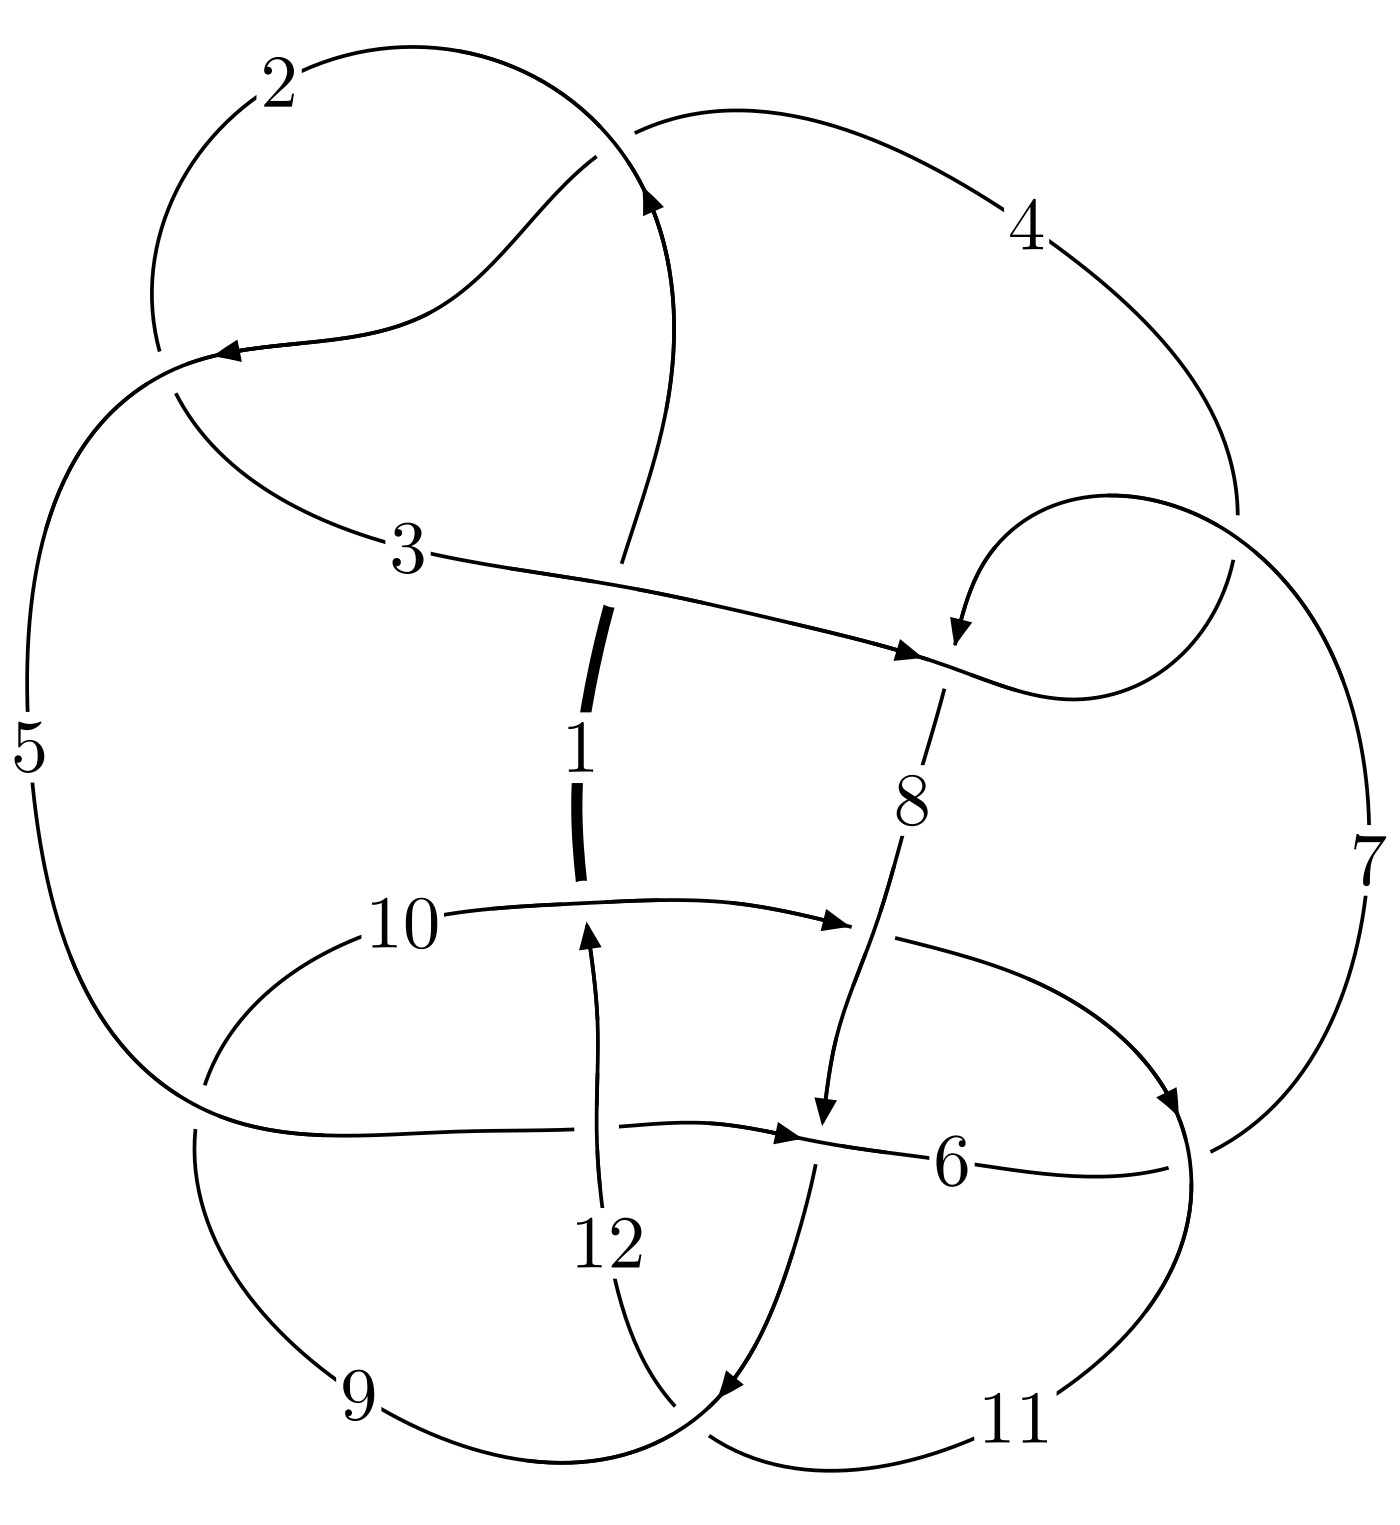
\includegraphics[width=112pt]{../../../GIT/diagram.site/Diagrams/png/2262_12n_0173.png}\\
\ \ \ A knot diagram\footnotemark}&
\allowdisplaybreaks
\textbf{Linearized knot diagam} \\
\cline{2-2}
 &
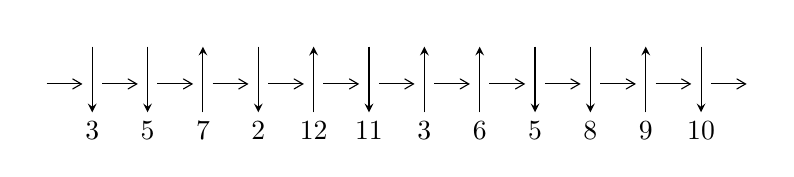
\begin{tikzpicture}[x=20pt, y=17pt]
	% nodes
	\node (C0) at (0, 0) {};
	\node (C1) at (1, 0) {};
	\node (C1U) at (1, +1) {};
	\node (C1D) at (1, -1) {3};

	\node (C2) at (2, 0) {};
	\node (C2U) at (2, +1) {};
	\node (C2D) at (2, -1) {5};

	\node (C3) at (3, 0) {};
	\node (C3U) at (3, +1) {};
	\node (C3D) at (3, -1) {7};

	\node (C4) at (4, 0) {};
	\node (C4U) at (4, +1) {};
	\node (C4D) at (4, -1) {2};

	\node (C5) at (5, 0) {};
	\node (C5U) at (5, +1) {};
	\node (C5D) at (5, -1) {12};

	\node (C6) at (6, 0) {};
	\node (C6U) at (6, +1) {};
	\node (C6D) at (6, -1) {11};

	\node (C7) at (7, 0) {};
	\node (C7U) at (7, +1) {};
	\node (C7D) at (7, -1) {3};

	\node (C8) at (8, 0) {};
	\node (C8U) at (8, +1) {};
	\node (C8D) at (8, -1) {6};

	\node (C9) at (9, 0) {};
	\node (C9U) at (9, +1) {};
	\node (C9D) at (9, -1) {5};

	\node (C10) at (10, 0) {};
	\node (C10U) at (10, +1) {};
	\node (C10D) at (10, -1) {8};

	\node (C11) at (11, 0) {};
	\node (C11U) at (11, +1) {};
	\node (C11D) at (11, -1) {9};

	\node (C12) at (12, 0) {};
	\node (C12U) at (12, +1) {};
	\node (C12D) at (12, -1) {10};
	\node (C13) at (13, 0) {};

	% arrows
	\draw[->,>={angle 60}]
	(C0) edge (C1) (C1) edge (C2) (C2) edge (C3) (C3) edge (C4) (C4) edge (C5) (C5) edge (C6) (C6) edge (C7) (C7) edge (C8) (C8) edge (C9) (C9) edge (C10) (C10) edge (C11) (C11) edge (C12) (C12) edge (C13) ;	\draw[->,>=stealth]
	(C1U) edge (C1D) (C2U) edge (C2D) (C3D) edge (C3U) (C4U) edge (C4D) (C5D) edge (C5U) (C6U) edge (C6D) (C7D) edge (C7U) (C8D) edge (C8U) (C9U) edge (C9D) (C10U) edge (C10D) (C11D) edge (C11U) (C12U) edge (C12D) ;
	\end{tikzpicture} \\
\hhline{~~} \\& 
\textbf{Solving Sequence} \\ \cline{2-2} 
 &
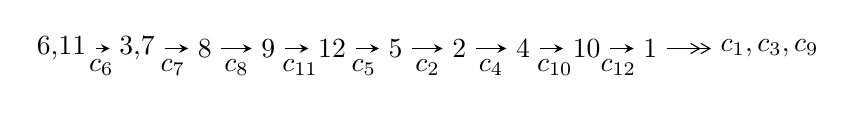
\begin{tikzpicture}[x=23pt, y=7pt]
	% node
	\node (A0) at (-1/8, 0) {6,11};
	\node (A1) at (17/16, 0) {3,7};
	\node (A2) at (17/8, 0) {8};
	\node (A3) at (25/8, 0) {9};
	\node (A4) at (33/8, 0) {12};
	\node (A5) at (41/8, 0) {5};
	\node (A6) at (49/8, 0) {2};
	\node (A7) at (57/8, 0) {4};
	\node (A8) at (65/8, 0) {10};
	\node (A9) at (73/8, 0) {1};
	\node (C1) at (1/2, -1) {$c_{6}$};
	\node (C2) at (13/8, -1) {$c_{7}$};
	\node (C3) at (21/8, -1) {$c_{8}$};
	\node (C4) at (29/8, -1) {$c_{11}$};
	\node (C5) at (37/8, -1) {$c_{5}$};
	\node (C6) at (45/8, -1) {$c_{2}$};
	\node (C7) at (53/8, -1) {$c_{4}$};
	\node (C8) at (61/8, -1) {$c_{10}$};
	\node (C9) at (69/8, -1) {$c_{12}$};
	\node (A10) at (11, 0) {$c_{1},c_{3},c_{9}$};

	% edge
	\draw[->,>=stealth]	
	(A0) edge (A1) (A1) edge (A2) (A2) edge (A3) (A3) edge (A4) (A4) edge (A5) (A5) edge (A6) (A6) edge (A7) (A7) edge (A8) (A8) edge (A9) ;
	\draw[->>,>={angle 60}]	
	(A9) edge (A10);
\end{tikzpicture} \\ 

\end{tabular} \\

\footnotetext{
The image of knot diagram is generated by the software ``\textbf{Draw programme}" developed by Andrew Bartholomew(\url{http://www.layer8.co.uk/maths/draw/index.htm\#Running-draw}), where we modified some parts for our purpose(\url{https://github.com/CATsTAILs/LinksPainter}).
}\phantom \\ \newline 
\centering \textbf{Ideals for irreducible components\footnotemark of $X_{\text{par}}$} 
 
\begin{align*}
I^u_{1}&=\langle 
-3.58032\times10^{67} u^{39}+2.06674\times10^{67} u^{38}+\cdots+9.73803\times10^{65} b-1.02729\times10^{69},\\
\phantom{I^u_{1}}&\phantom{= \langle  }5.45075\times10^{69} u^{39}-3.75387\times10^{69} u^{38}+\cdots+1.65547\times10^{67} a+1.34484\times10^{71},\;u^{40}-4 u^{38}+\cdots+97 u+17\rangle \\
I^u_{2}&=\langle 
9.27676\times10^{169} u^{45}-2.27749\times10^{170} u^{44}+\cdots+9.75406\times10^{172} b+4.16059\times10^{173},\\
\phantom{I^u_{2}}&\phantom{= \langle  }9.42080\times10^{173} u^{45}-2.43360\times10^{174} u^{44}+\cdots+2.48046\times10^{176} a+3.47623\times10^{177},\\
\phantom{I^u_{2}}&\phantom{= \langle  }u^{46}-2 u^{45}+\cdots+9446 u+2543\rangle \\
I^u_{3}&=\langle 
u^3+3 u^2+4 b+2 u+1,\;-3 u^3- u^2+4 a-2 u+5,\;u^4+u^2- u+1\rangle \\
I^u_{4}&=\langle 
-4 u^{14}-2 u^{13}+\cdots+b-5,\\
\phantom{I^u_{4}}&\phantom{= \langle  }-2 u^{14}- u^{13}+5 u^{12}-3 u^{11}-10 u^{10}+11 u^9+10 u^8-14 u^7-3 u^6+14 u^5+u^4-8 u^3+u^2+a+3 u-1,\\
\phantom{I^u_{4}}&\phantom{= \langle  }u^{15}-3 u^{13}+3 u^{12}+5 u^{11}-9 u^{10}-3 u^9+12 u^8-2 u^7-11 u^6+4 u^5+7 u^4-5 u^3-2 u^2+3 u-1\rangle \\
I^u_{5}&=\langle 
- u^5- u^4-2 u^3-2 u^2+b- u-1,\;- u^5-2 u^3- u^2+a-2 u-2,\;u^6+u^5+2 u^4+2 u^3+2 u^2+2 u+1\rangle \\
\\
\end{align*}
\raggedright * 5 irreducible components of $\dim_{\mathbb{C}}=0$, with total 111 representations.\\
\footnotetext{All coefficients of polynomials are rational numbers. But the coefficients are sometimes approximated in decimal forms when there is not enough margin.}
\newpage
\renewcommand{\arraystretch}{1}
\centering \section*{I. $I^u_{1}= \langle -3.58\times10^{67} u^{39}+2.07\times10^{67} u^{38}+\cdots+9.74\times10^{65} b-1.03\times10^{69},\;5.45\times10^{69} u^{39}-3.75\times10^{69} u^{38}+\cdots+1.66\times10^{67} a+1.34\times10^{71},\;u^{40}-4 u^{38}+\cdots+97 u+17 \rangle$}
\flushleft \textbf{(i) Arc colorings}\\
\begin{tabular}{m{7pt} m{180pt} m{7pt} m{180pt} }
\flushright $a_{6}=$&$\begin{pmatrix}1\\0\end{pmatrix}$ \\
\flushright $a_{11}=$&$\begin{pmatrix}0\\u\end{pmatrix}$ \\
\flushright $a_{3}=$&$\begin{pmatrix}-329.258 u^{39}+226.756 u^{38}+\cdots-34572.1 u-8123.67\\36.7664 u^{39}-21.2234 u^{38}+\cdots+4276.56 u+1054.93\end{pmatrix}$ \\
\flushright $a_{7}=$&$\begin{pmatrix}1\\u^2\end{pmatrix}$ \\
\flushright $a_{8}=$&$\begin{pmatrix}-79.7827 u^{39}+49.4021 u^{38}+\cdots-8924.80 u-2162.21\\-83.0595 u^{39}+59.0553 u^{38}+\cdots-8544.73 u-1992.63\end{pmatrix}$ \\
\flushright $a_{9}=$&$\begin{pmatrix}-162.842 u^{39}+108.457 u^{38}+\cdots-17469.5 u-4154.84\\-83.0595 u^{39}+59.0553 u^{38}+\cdots-8544.73 u-1992.63\end{pmatrix}$ \\
\flushright $a_{12}=$&$\begin{pmatrix}-398.430 u^{39}+268.461 u^{38}+\cdots-42420.9 u-10043.8\\-83.0595 u^{39}+59.0553 u^{38}+\cdots-8544.73 u-1992.63\end{pmatrix}$ \\
\flushright $a_{5}=$&$\begin{pmatrix}8.75622 u^{39}-10.8797 u^{38}+\cdots+451.374 u+56.6766\\-120.738 u^{39}+80.3482 u^{38}+\cdots-12927.2 u-3059.02\end{pmatrix}$ \\
\flushright $a_{2}=$&$\begin{pmatrix}-90.2726 u^{39}+62.6721 u^{38}+\cdots-9459.34 u-2231.28\\87.9281 u^{39}-59.6344 u^{38}+\cdots+9289.11 u+2178.55\end{pmatrix}$ \\
\flushright $a_{4}=$&$\begin{pmatrix}136.341 u^{39}-97.9644 u^{38}+\cdots+13897.5 u+3213.89\\-122.755 u^{39}+78.6483 u^{38}+\cdots-13489.8 u-3244.38\end{pmatrix}$ \\
\flushright $a_{10}=$&$\begin{pmatrix}-151.962 u^{39}+97.3994 u^{38}+\cdots-16676.8 u-4005.99\\-163.408 u^{39}+112.006 u^{38}+\cdots-17197.3 u-4045.18\end{pmatrix}$ \\
\flushright $a_{1}=$&$\begin{pmatrix}-107.859 u^{39}+79.5764 u^{38}+\cdots-10793.0 u-2477.92\\152.528 u^{39}-100.948 u^{38}+\cdots+16405.7 u+3896.33\end{pmatrix}$\\&\end{tabular}
\flushleft \textbf{(ii) Obstruction class $= -1$}\\~\\
\flushleft \textbf{(iii) Cusp Shapes $= -185.230 u^{39}+123.975 u^{38}+\cdots-19743.3 u-4644.59$}\\~\\
\newpage\renewcommand{\arraystretch}{1}
\flushleft \textbf{(iv) u-Polynomials at the component}\newline \\
\begin{tabular}{m{50pt}|m{274pt}}
Crossings & \hspace{64pt}u-Polynomials at each crossing \\
\hline $$\begin{aligned}c_{1}\end{aligned}$$&$\begin{aligned}
&u^{40}+41 u^{39}+\cdots+8641 u+256
\end{aligned}$\\
\hline $$\begin{aligned}c_{2},c_{4}\end{aligned}$$&$\begin{aligned}
&u^{40}-7 u^{39}+\cdots-81 u+16
\end{aligned}$\\
\hline $$\begin{aligned}c_{3},c_{7}\end{aligned}$$&$\begin{aligned}
&u^{40}-5 u^{39}+\cdots+1632 u+256
\end{aligned}$\\
\hline $$\begin{aligned}c_{5},c_{8}\end{aligned}$$&$\begin{aligned}
&u^{40}+u^{39}+\cdots+2 u+1
\end{aligned}$\\
\hline $$\begin{aligned}c_{6},c_{9}\end{aligned}$$&$\begin{aligned}
&u^{40}-4 u^{38}+\cdots-97 u+17
\end{aligned}$\\
\hline $$\begin{aligned}c_{10},c_{12}\end{aligned}$$&$\begin{aligned}
&u^{40}+4 u^{39}+\cdots-3 u+1
\end{aligned}$\\
\hline $$\begin{aligned}c_{11}\end{aligned}$$&$\begin{aligned}
&u^{40}+25 u^{39}+\cdots+36 u+4
\end{aligned}$\\
\hline
\end{tabular}\\~\\
\newpage\renewcommand{\arraystretch}{1}
\flushleft \textbf{(v) Riley Polynomials at the component}\newline \\
\begin{tabular}{m{50pt}|m{274pt}}
Crossings & \hspace{64pt}Riley Polynomials at each crossing \\
\hline $$\begin{aligned}c_{1}\end{aligned}$$&$\begin{aligned}
&y^{40}-77 y^{39}+\cdots-6662529 y+65536
\end{aligned}$\\
\hline $$\begin{aligned}c_{2},c_{4}\end{aligned}$$&$\begin{aligned}
&y^{40}-41 y^{39}+\cdots-8641 y+256
\end{aligned}$\\
\hline $$\begin{aligned}c_{3},c_{7}\end{aligned}$$&$\begin{aligned}
&y^{40}+27 y^{39}+\cdots-226304 y+65536
\end{aligned}$\\
\hline $$\begin{aligned}c_{5},c_{8}\end{aligned}$$&$\begin{aligned}
&y^{40}+17 y^{39}+\cdots+40 y+1
\end{aligned}$\\
\hline $$\begin{aligned}c_{6},c_{9}\end{aligned}$$&$\begin{aligned}
&y^{40}-8 y^{39}+\cdots-4275 y+289
\end{aligned}$\\
\hline $$\begin{aligned}c_{10},c_{12}\end{aligned}$$&$\begin{aligned}
&y^{40}-40 y^{39}+\cdots-15 y+1
\end{aligned}$\\
\hline $$\begin{aligned}c_{11}\end{aligned}$$&$\begin{aligned}
&y^{40}- y^{39}+\cdots+1144 y+16
\end{aligned}$\\
\hline
\end{tabular}\\~\\
\newpage\flushleft \textbf{(vi) Complex Volumes and Cusp Shapes}
$$\begin{array}{c|c|c}  
\text{Solutions to }I^u_{1}& \I (\text{vol} + \sqrt{-1}CS) & \text{Cusp shape}\\
 \hline 
\begin{aligned}
u &= -0.916795 + 0.271284 I \\
a &= \phantom{-}0.07185 - 2.25689 I \\
b &= -0.886132 - 0.556013 I\end{aligned}
 & -4.61460 + 4.21677 I & -10.36400 - 7.96016 I \\ \hline\begin{aligned}
u &= -0.916795 - 0.271284 I \\
a &= \phantom{-}0.07185 + 2.25689 I \\
b &= -0.886132 + 0.556013 I\end{aligned}
 & -4.61460 - 4.21677 I & -10.36400 + 7.96016 I \\ \hline\begin{aligned}
u &= -0.257747 + 1.059350 I \\
a &= -1.51427 + 1.70732 I \\
b &= \phantom{-}2.53555 - 1.59062 I\end{aligned}
 & -2.65950 + 0.01537 I & -10.44302 + 0.45727 I \\ \hline\begin{aligned}
u &= -0.257747 - 1.059350 I \\
a &= -1.51427 - 1.70732 I \\
b &= \phantom{-}2.53555 + 1.59062 I\end{aligned}
 & -2.65950 - 0.01537 I & -10.44302 - 0.45727 I \\ \hline\begin{aligned}
u &= -0.773206 + 0.447559 I \\
a &= \phantom{-}0.294992 - 0.155460 I \\
b &= \phantom{-}1.237270 + 0.037085 I\end{aligned}
 & \phantom{-}1.37570 + 6.93076 I & -8.7508 - 11.5757 I \\ \hline\begin{aligned}
u &= -0.773206 - 0.447559 I \\
a &= \phantom{-}0.294992 + 0.155460 I \\
b &= \phantom{-}1.237270 - 0.037085 I\end{aligned}
 & \phantom{-}1.37570 - 6.93076 I & -8.7508 + 11.5757 I \\ \hline\begin{aligned}
u &= \phantom{-}0.843869 + 0.116958 I \\
a &= \phantom{-}0.699504 + 0.268479 I \\
b &= -0.806806 + 0.392167 I\end{aligned}
 & -6.65685 - 1.58265 I & -10.51643 + 4.50982 I \\ \hline\begin{aligned}
u &= \phantom{-}0.843869 - 0.116958 I \\
a &= \phantom{-}0.699504 - 0.268479 I \\
b &= -0.806806 - 0.392167 I\end{aligned}
 & -6.65685 + 1.58265 I & -10.51643 - 4.50982 I \\ \hline\begin{aligned}
u &= -0.742457 + 0.416076 I \\
a &= -1.13504 + 1.53730 I \\
b &= -0.146732 - 0.117931 I\end{aligned}
 & -10.74610 + 5.03761 I & -8.95297 - 0.57470 I \\ \hline\begin{aligned}
u &= -0.742457 - 0.416076 I \\
a &= -1.13504 - 1.53730 I \\
b &= -0.146732 + 0.117931 I\end{aligned}
 & -10.74610 - 5.03761 I & -8.95297 + 0.57470 I\\
 \hline 
 \end{array}$$\newpage$$\begin{array}{c|c|c}  
\text{Solutions to }I^u_{1}& \I (\text{vol} + \sqrt{-1}CS) & \text{Cusp shape}\\
 \hline 
\begin{aligned}
u &= -0.596745 + 1.034040 I \\
a &= \phantom{-}0.0958413 - 0.0250611 I \\
b &= \phantom{-}0.457567 - 0.044691 I\end{aligned}
 & \phantom{-}1.35612 + 7.74333 I & \phantom{-}9.28204 - 10.17690 I \\ \hline\begin{aligned}
u &= -0.596745 - 1.034040 I \\
a &= \phantom{-}0.0958413 + 0.0250611 I \\
b &= \phantom{-}0.457567 + 0.044691 I\end{aligned}
 & \phantom{-}1.35612 - 7.74333 I & \phantom{-}9.28204 + 10.17690 I \\ \hline\begin{aligned}
u &= \phantom{-}0.515825 + 1.095850 I \\
a &= \phantom{-}0.699738 + 0.145025 I \\
b &= -0.618119 - 0.598353 I\end{aligned}
 & -5.33600 - 3.23521 I & \phantom{-0.000000 } 0 \\ \hline\begin{aligned}
u &= \phantom{-}0.515825 - 1.095850 I \\
a &= \phantom{-}0.699738 - 0.145025 I \\
b &= -0.618119 + 0.598353 I\end{aligned}
 & -5.33600 + 3.23521 I & \phantom{-0.000000 } 0 \\ \hline\begin{aligned}
u &= \phantom{-}0.297740 + 0.729548 I \\
a &= -0.726912 - 0.545199 I \\
b &= \phantom{-}0.205553 + 0.589406 I\end{aligned}
 & \phantom{-}0.08293 - 1.53752 I & \phantom{-}0.71639 + 4.76389 I \\ \hline\begin{aligned}
u &= \phantom{-}0.297740 - 0.729548 I \\
a &= -0.726912 + 0.545199 I \\
b &= \phantom{-}0.205553 - 0.589406 I\end{aligned}
 & \phantom{-}0.08293 + 1.53752 I & \phantom{-}0.71639 - 4.76389 I \\ \hline\begin{aligned}
u &= \phantom{-}0.594134 + 0.510868 I \\
a &= -0.461994 + 0.161353 I \\
b &= \phantom{-}0.337579 - 0.191190 I\end{aligned}
 & -1.25513 - 1.56952 I & -2.17390 + 4.23177 I \\ \hline\begin{aligned}
u &= \phantom{-}0.594134 - 0.510868 I \\
a &= -0.461994 - 0.161353 I \\
b &= \phantom{-}0.337579 + 0.191190 I\end{aligned}
 & -1.25513 + 1.56952 I & -2.17390 - 4.23177 I \\ \hline\begin{aligned}
u &= -1.178420 + 0.383003 I \\
a &= -0.27016 + 1.72025 I \\
b &= \phantom{-}0.672757 + 0.873454 I\end{aligned}
 & -11.7135 + 8.0385 I & -13.2209 - 9.1027 I \\ \hline\begin{aligned}
u &= -1.178420 - 0.383003 I \\
a &= -0.27016 - 1.72025 I \\
b &= \phantom{-}0.672757 - 0.873454 I\end{aligned}
 & -11.7135 - 8.0385 I & -13.2209 + 9.1027 I\\
 \hline 
 \end{array}$$\newpage$$\begin{array}{c|c|c}  
\text{Solutions to }I^u_{1}& \I (\text{vol} + \sqrt{-1}CS) & \text{Cusp shape}\\
 \hline 
\begin{aligned}
u &= \phantom{-}0.668836 + 0.264877 I \\
a &= \phantom{-}0.282272 + 1.160020 I \\
b &= \phantom{-}0.135893 - 0.315911 I\end{aligned}
 & -1.90192 + 1.40153 I & -6.20748 - 1.19828 I \\ \hline\begin{aligned}
u &= \phantom{-}0.668836 - 0.264877 I \\
a &= \phantom{-}0.282272 - 1.160020 I \\
b &= \phantom{-}0.135893 + 0.315911 I\end{aligned}
 & -1.90192 - 1.40153 I & -6.20748 + 1.19828 I \\ \hline\begin{aligned}
u &= -0.679465 + 0.012974 I \\
a &= \phantom{-}0.90700 - 2.42772 I \\
b &= \phantom{-}0.690272 + 0.025224 I\end{aligned}
 & -4.35694 + 0.92822 I & -9.14930 + 0.28573 I \\ \hline\begin{aligned}
u &= -0.679465 - 0.012974 I \\
a &= \phantom{-}0.90700 + 2.42772 I \\
b &= \phantom{-}0.690272 - 0.025224 I\end{aligned}
 & -4.35694 - 0.92822 I & -9.14930 - 0.28573 I \\ \hline\begin{aligned}
u &= -0.423175 + 0.521589 I \\
a &= \phantom{-}1.35188 + 1.41277 I \\
b &= \phantom{-}1.03242 - 1.13997 I\end{aligned}
 & -2.35252 + 0.61317 I & -4.61633 + 3.05486 I \\ \hline\begin{aligned}
u &= -0.423175 - 0.521589 I \\
a &= \phantom{-}1.35188 - 1.41277 I \\
b &= \phantom{-}1.03242 + 1.13997 I\end{aligned}
 & -2.35252 - 0.61317 I & -4.61633 - 3.05486 I \\ \hline\begin{aligned}
u &= -0.663180 + 0.080866 I \\
a &= -0.505742 + 0.206401 I \\
b &= -1.384640 - 0.132216 I\end{aligned}
 & \phantom{-}2.64301 + 1.48294 I & -4.81453 + 7.72547 I \\ \hline\begin{aligned}
u &= -0.663180 - 0.080866 I \\
a &= -0.505742 - 0.206401 I \\
b &= -1.384640 + 0.132216 I\end{aligned}
 & \phantom{-}2.64301 - 1.48294 I & -4.81453 - 7.72547 I \\ \hline\begin{aligned}
u &= \phantom{-}1.31926 + 0.81503 I \\
a &= -0.254068 - 1.123980 I \\
b &= \phantom{-}2.08311 - 0.15702 I\end{aligned}
 & -5.42435 - 5.89974 I & \phantom{-0.000000 } 0 \\ \hline\begin{aligned}
u &= \phantom{-}1.31926 - 0.81503 I \\
a &= -0.254068 + 1.123980 I \\
b &= \phantom{-}2.08311 + 0.15702 I\end{aligned}
 & -5.42435 + 5.89974 I & \phantom{-0.000000 } 0\\
 \hline 
 \end{array}$$\newpage$$\begin{array}{c|c|c}  
\text{Solutions to }I^u_{1}& \I (\text{vol} + \sqrt{-1}CS) & \text{Cusp shape}\\
 \hline 
\begin{aligned}
u &= -1.33509 + 1.00004 I \\
a &= -0.103766 + 0.191805 I \\
b &= -1.191910 + 0.700889 I\end{aligned}
 & -7.28442 + 9.37900 I & \phantom{-0.000000 } 0 \\ \hline\begin{aligned}
u &= -1.33509 - 1.00004 I \\
a &= -0.103766 - 0.191805 I \\
b &= -1.191910 - 0.700889 I\end{aligned}
 & -7.28442 - 9.37900 I & \phantom{-0.000000 } 0 \\ \hline\begin{aligned}
u &= \phantom{-}1.64955 + 0.34859 I \\
a &= \phantom{-}0.041797 + 0.918280 I \\
b &= -1.41260 + 0.58964 I\end{aligned}
 & -14.3131 - 1.3284 I & \phantom{-0.000000 } 0 \\ \hline\begin{aligned}
u &= \phantom{-}1.64955 - 0.34859 I \\
a &= \phantom{-}0.041797 - 0.918280 I \\
b &= -1.41260 - 0.58964 I\end{aligned}
 & -14.3131 + 1.3284 I & \phantom{-0.000000 } 0 \\ \hline\begin{aligned}
u &= \phantom{-}1.25011 + 1.13972 I \\
a &= \phantom{-}0.537152 + 1.115220 I \\
b &= -2.58218 + 0.30646 I\end{aligned}
 & -4.50733 - 12.55940 I & \phantom{-0.000000 } 0 \\ \hline\begin{aligned}
u &= \phantom{-}1.25011 - 1.13972 I \\
a &= \phantom{-}0.537152 - 1.115220 I \\
b &= -2.58218 - 0.30646 I\end{aligned}
 & -4.50733 + 12.55940 I & \phantom{-0.000000 } 0 \\ \hline\begin{aligned}
u &= -0.82513 + 1.61273 I \\
a &= \phantom{-}0.619679 - 0.520496 I \\
b &= -2.49695 + 0.94026 I\end{aligned}
 & -10.55600 + 0.42655 I & \phantom{-0.000000 } 0 \\ \hline\begin{aligned}
u &= -0.82513 - 1.61273 I \\
a &= \phantom{-}0.619679 + 0.520496 I \\
b &= -2.49695 - 0.94026 I\end{aligned}
 & -10.55600 - 0.42655 I & \phantom{-0.000000 } 0 \\ \hline\begin{aligned}
u &= \phantom{-}1.25209 + 1.40579 I \\
a &= -0.710628 - 0.936920 I \\
b &= \phantom{-}2.76309 - 0.57698 I\end{aligned}
 & -11.2981 - 17.8760 I & \phantom{-0.000000 } 0 \\ \hline\begin{aligned}
u &= \phantom{-}1.25209 - 1.40579 I \\
a &= -0.710628 + 0.936920 I \\
b &= \phantom{-}2.76309 + 0.57698 I\end{aligned}
 & -11.2981 + 17.8760 I & \phantom{-0.000000 } 0\\
 \hline 
 \end{array}$$\newpage\newpage\renewcommand{\arraystretch}{1}
\centering \section*{II. $I^u_{2}= \langle 9.28\times10^{169} u^{45}-2.28\times10^{170} u^{44}+\cdots+9.75\times10^{172} b+4.16\times10^{173},\;9.42\times10^{173} u^{45}-2.43\times10^{174} u^{44}+\cdots+2.48\times10^{176} a+3.48\times10^{177},\;u^{46}-2 u^{45}+\cdots+9446 u+2543 \rangle$}
\flushleft \textbf{(i) Arc colorings}\\
\begin{tabular}{m{7pt} m{180pt} m{7pt} m{180pt} }
\flushright $a_{6}=$&$\begin{pmatrix}1\\0\end{pmatrix}$ \\
\flushright $a_{11}=$&$\begin{pmatrix}0\\u\end{pmatrix}$ \\
\flushright $a_{3}=$&$\begin{pmatrix}-0.00379801 u^{45}+0.00981109 u^{44}+\cdots-43.1222 u-14.0145\\-0.000951066 u^{45}+0.00233492 u^{44}+\cdots-8.80677 u-4.26549\end{pmatrix}$ \\
\flushright $a_{7}=$&$\begin{pmatrix}1\\u^2\end{pmatrix}$ \\
\flushright $a_{8}=$&$\begin{pmatrix}0.000716237 u^{45}-0.00105546 u^{44}+\cdots+4.58476 u+9.05145\\0.00144541 u^{45}-0.00363803 u^{44}+\cdots+12.3847 u+6.56682\end{pmatrix}$ \\
\flushright $a_{9}=$&$\begin{pmatrix}0.00216165 u^{45}-0.00469349 u^{44}+\cdots+16.9695 u+15.6183\\0.00144541 u^{45}-0.00363803 u^{44}+\cdots+12.3847 u+6.56682\end{pmatrix}$ \\
\flushright $a_{12}=$&$\begin{pmatrix}-0.00398318 u^{45}+0.00931129 u^{44}+\cdots-34.5587 u-20.7912\\-0.000496329 u^{45}+0.000994531 u^{44}+\cdots-6.30884 u-5.67547\end{pmatrix}$ \\
\flushright $a_{5}=$&$\begin{pmatrix}0.00412015 u^{45}-0.0103795 u^{44}+\cdots+41.9047 u+14.6677\\0.000976621 u^{45}-0.00236780 u^{44}+\cdots+11.0461 u+5.89430\end{pmatrix}$ \\
\flushright $a_{2}=$&$\begin{pmatrix}-0.00289423 u^{45}+0.00709969 u^{44}+\cdots-29.5330 u-10.4974\\-0.000537120 u^{45}+0.00126553 u^{44}+\cdots-6.34240 u-3.78873\end{pmatrix}$ \\
\flushright $a_{4}=$&$\begin{pmatrix}0.00382997 u^{45}-0.00995571 u^{44}+\cdots+40.6638 u+12.6470\\0.00116221 u^{45}-0.00292917 u^{44}+\cdots+9.48770 u+4.47069\end{pmatrix}$ \\
\flushright $a_{10}=$&$\begin{pmatrix}-0.00461706 u^{45}+0.0113680 u^{44}+\cdots-34.2999 u-16.9762\\0.00113021 u^{45}-0.00305123 u^{44}+\cdots+8.04999 u+1.86051\end{pmatrix}$ \\
\flushright $a_{1}=$&$\begin{pmatrix}-0.00527624 u^{45}+0.0130113 u^{44}+\cdots-46.7854 u-17.7735\\0.000580431 u^{45}-0.00159375 u^{44}+\cdots+1.15606 u-0.758198\end{pmatrix}$\\&\end{tabular}
\flushleft \textbf{(ii) Obstruction class $= -1$}\\~\\
\flushleft \textbf{(iii) Cusp Shapes $= 0.00495504 u^{45}-0.00970261 u^{44}+\cdots+38.8323 u+37.7445$}\\~\\
\newpage\renewcommand{\arraystretch}{1}
\flushleft \textbf{(iv) u-Polynomials at the component}\newline \\
\begin{tabular}{m{50pt}|m{274pt}}
Crossings & \hspace{64pt}u-Polynomials at each crossing \\
\hline $$\begin{aligned}c_{1}\end{aligned}$$&$\begin{aligned}
&(u^{23}+26 u^{22}+\cdots-7 u+1)^{2}
\end{aligned}$\\
\hline $$\begin{aligned}c_{2},c_{4}\end{aligned}$$&$\begin{aligned}
&(u^{23}-4 u^{22}+\cdots-3 u-1)^{2}
\end{aligned}$\\
\hline $$\begin{aligned}c_{3},c_{7}\end{aligned}$$&$\begin{aligned}
&(u^{23}+3 u^{22}+\cdots+36 u-8)^{2}
\end{aligned}$\\
\hline $$\begin{aligned}c_{5},c_{8}\end{aligned}$$&$\begin{aligned}
&u^{46}+6 u^{45}+\cdots+116 u+17
\end{aligned}$\\
\hline $$\begin{aligned}c_{6},c_{9}\end{aligned}$$&$\begin{aligned}
&u^{46}+2 u^{45}+\cdots-9446 u+2543
\end{aligned}$\\
\hline $$\begin{aligned}c_{10},c_{12}\end{aligned}$$&$\begin{aligned}
&u^{46}-3 u^{44}+\cdots-76140 u+32521
\end{aligned}$\\
\hline $$\begin{aligned}c_{11}\end{aligned}$$&$\begin{aligned}
&(u^{23}-10 u^{22}+\cdots+4 u^2+1)^{2}
\end{aligned}$\\
\hline
\end{tabular}\\~\\
\newpage\renewcommand{\arraystretch}{1}
\flushleft \textbf{(v) Riley Polynomials at the component}\newline \\
\begin{tabular}{m{50pt}|m{274pt}}
Crossings & \hspace{64pt}Riley Polynomials at each crossing \\
\hline $$\begin{aligned}c_{1}\end{aligned}$$&$\begin{aligned}
&(y^{23}-54 y^{22}+\cdots-215 y-1)^{2}
\end{aligned}$\\
\hline $$\begin{aligned}c_{2},c_{4}\end{aligned}$$&$\begin{aligned}
&(y^{23}-26 y^{22}+\cdots-7 y-1)^{2}
\end{aligned}$\\
\hline $$\begin{aligned}c_{3},c_{7}\end{aligned}$$&$\begin{aligned}
&(y^{23}+21 y^{22}+\cdots-48 y-64)^{2}
\end{aligned}$\\
\hline $$\begin{aligned}c_{5},c_{8}\end{aligned}$$&$\begin{aligned}
&y^{46}-10 y^{45}+\cdots+3136 y+289
\end{aligned}$\\
\hline $$\begin{aligned}c_{6},c_{9}\end{aligned}$$&$\begin{aligned}
&y^{46}-10 y^{45}+\cdots-111757896 y+6466849
\end{aligned}$\\
\hline $$\begin{aligned}c_{10},c_{12}\end{aligned}$$&$\begin{aligned}
&y^{46}-6 y^{45}+\cdots+636394872 y+1057615441
\end{aligned}$\\
\hline $$\begin{aligned}c_{11}\end{aligned}$$&$\begin{aligned}
&(y^{23}+20 y^{21}+\cdots-8 y-1)^{2}
\end{aligned}$\\
\hline
\end{tabular}\\~\\
\newpage\flushleft \textbf{(vi) Complex Volumes and Cusp Shapes}
$$\begin{array}{c|c|c}  
\text{Solutions to }I^u_{2}& \I (\text{vol} + \sqrt{-1}CS) & \text{Cusp shape}\\
 \hline 
\begin{aligned}
u &= \phantom{-}0.938998 + 0.344976 I \\
a &= -2.24368 + 0.34394 I \\
b &= -2.40240 - 0.99716 I\end{aligned}
 & -1.23158 - 3.46001 I & -0.93966 + 11.94434 I \\ \hline\begin{aligned}
u &= \phantom{-}0.938998 - 0.344976 I \\
a &= -2.24368 - 0.34394 I \\
b &= -2.40240 + 0.99716 I\end{aligned}
 & -1.23158 + 3.46001 I & -0.93966 - 11.94434 I \\ \hline\begin{aligned}
u &= \phantom{-}0.381487 + 0.925362 I \\
a &= \phantom{-}0.036904 - 0.397055 I \\
b &= -0.308362 + 0.632471 I\end{aligned}
 & \phantom{-}0.22577 - 2.35596 I & \phantom{-}1.37102 + 5.00512 I \\ \hline\begin{aligned}
u &= \phantom{-}0.381487 - 0.925362 I \\
a &= \phantom{-}0.036904 + 0.397055 I \\
b &= -0.308362 - 0.632471 I\end{aligned}
 & \phantom{-}0.22577 + 2.35596 I & \phantom{-}1.37102 - 5.00512 I \\ \hline\begin{aligned}
u &= -0.662967 + 0.741919 I \\
a &= -0.882738 + 0.492316 I \\
b &= \phantom{-}0.019759 + 1.137980 I\end{aligned}
 & \phantom{-}0.22577 - 2.35596 I & \phantom{-}1.37102 + 5.00512 I \\ \hline\begin{aligned}
u &= -0.662967 - 0.741919 I \\
a &= -0.882738 - 0.492316 I \\
b &= \phantom{-}0.019759 - 1.137980 I\end{aligned}
 & \phantom{-}0.22577 + 2.35596 I & \phantom{-}1.37102 - 5.00512 I \\ \hline\begin{aligned}
u &= -0.776430 + 0.599101 I \\
a &= \phantom{-}0.64174 - 1.41107 I \\
b &= -0.331275 + 0.637663 I\end{aligned}
 & -9.93186 + 9.38993 I & -5.00822 - 8.89816 I \\ \hline\begin{aligned}
u &= -0.776430 - 0.599101 I \\
a &= \phantom{-}0.64174 + 1.41107 I \\
b &= -0.331275 - 0.637663 I\end{aligned}
 & -9.93186 - 9.38993 I & -5.00822 + 8.89816 I \\ \hline\begin{aligned}
u &= -0.347658 + 0.962709 I \\
a &= -0.094250 - 0.137661 I \\
b &= -0.617430 + 0.174037 I\end{aligned}
 & \phantom{-}3.29942\phantom{ +0.000000I} & \phantom{-}11.64034 + 0. I\phantom{ +0.000000I} \\ \hline\begin{aligned}
u &= -0.347658 - 0.962709 I \\
a &= -0.094250 + 0.137661 I \\
b &= -0.617430 - 0.174037 I\end{aligned}
 & \phantom{-}3.29942\phantom{ +0.000000I} & \phantom{-}11.64034 + 0. I\phantom{ +0.000000I}\\
 \hline 
 \end{array}$$\newpage$$\begin{array}{c|c|c}  
\text{Solutions to }I^u_{2}& \I (\text{vol} + \sqrt{-1}CS) & \text{Cusp shape}\\
 \hline 
\begin{aligned}
u &= \phantom{-}0.363894 + 0.859272 I \\
a &= \phantom{-}0.961328 - 0.913318 I \\
b &= \phantom{-}0.081085 + 0.409837 I\end{aligned}
 & \phantom{-}0.07682 - 4.67687 I & -2.82043 + 11.56965 I \\ \hline\begin{aligned}
u &= \phantom{-}0.363894 - 0.859272 I \\
a &= \phantom{-}0.961328 + 0.913318 I \\
b &= \phantom{-}0.081085 - 0.409837 I\end{aligned}
 & \phantom{-}0.07682 + 4.67687 I & -2.82043 - 11.56965 I \\ \hline\begin{aligned}
u &= -0.576444 + 0.916663 I \\
a &= -3.57574 + 2.35289 I \\
b &= \phantom{-}3.83467 + 2.38953 I\end{aligned}
 & -1.23158 + 3.46001 I & -0.93966 - 11.94434 I \\ \hline\begin{aligned}
u &= -0.576444 - 0.916663 I \\
a &= -3.57574 - 2.35289 I \\
b &= \phantom{-}3.83467 - 2.38953 I\end{aligned}
 & -1.23158 - 3.46001 I & -0.93966 + 11.94434 I \\ \hline\begin{aligned}
u &= \phantom{-}0.091395 + 1.210170 I \\
a &= -0.143737 + 0.825821 I \\
b &= -0.195131 + 0.246758 I\end{aligned}
 & -6.90053 - 6.33030 I & -5.55743 + 6.60020 I \\ \hline\begin{aligned}
u &= \phantom{-}0.091395 - 1.210170 I \\
a &= -0.143737 - 0.825821 I \\
b &= -0.195131 - 0.246758 I\end{aligned}
 & -6.90053 + 6.33030 I & -5.55743 - 6.60020 I \\ \hline\begin{aligned}
u &= -0.642034 + 0.452369 I \\
a &= -0.21983 + 1.87152 I \\
b &= \phantom{-}1.23526 - 0.94866 I\end{aligned}
 & -4.25470 + 2.83401 I & -16.2136 - 5.6542 I \\ \hline\begin{aligned}
u &= -0.642034 - 0.452369 I \\
a &= -0.21983 - 1.87152 I \\
b &= \phantom{-}1.23526 + 0.94866 I\end{aligned}
 & -4.25470 - 2.83401 I & -16.2136 + 5.6542 I \\ \hline\begin{aligned}
u &= \phantom{-}0.669574 + 1.086330 I \\
a &= -0.208906 - 0.373689 I \\
b &= \phantom{-}0.927797 + 0.477174 I\end{aligned}
 & \phantom{-}0.78715 - 2.82758 I & \phantom{-}2.28819 - 1.37730 I \\ \hline\begin{aligned}
u &= \phantom{-}0.669574 - 1.086330 I \\
a &= -0.208906 + 0.373689 I \\
b &= \phantom{-}0.927797 - 0.477174 I\end{aligned}
 & \phantom{-}0.78715 + 2.82758 I & \phantom{-}2.28819 + 1.37730 I\\
 \hline 
 \end{array}$$\newpage$$\begin{array}{c|c|c}  
\text{Solutions to }I^u_{2}& \I (\text{vol} + \sqrt{-1}CS) & \text{Cusp shape}\\
 \hline 
\begin{aligned}
u &= -1.046560 + 0.783431 I \\
a &= \phantom{-}0.59848 - 1.43771 I \\
b &= -1.59045 + 0.05140 I\end{aligned}
 & -12.8626 + 6.8428 I & -11.21020 - 4.32033 I \\ \hline\begin{aligned}
u &= -1.046560 - 0.783431 I \\
a &= \phantom{-}0.59848 + 1.43771 I \\
b &= -1.59045 - 0.05140 I\end{aligned}
 & -12.8626 - 6.8428 I & -11.21020 + 4.32033 I \\ \hline\begin{aligned}
u &= \phantom{-}0.625428 + 0.116207 I \\
a &= -0.714645 + 0.198843 I \\
b &= \phantom{-}1.353840 - 0.397532 I\end{aligned}
 & -5.87167 + 0.65487 I & -18.5419 - 8.9539 I \\ \hline\begin{aligned}
u &= \phantom{-}0.625428 - 0.116207 I \\
a &= -0.714645 - 0.198843 I \\
b &= \phantom{-}1.353840 + 0.397532 I\end{aligned}
 & -5.87167 - 0.65487 I & -18.5419 + 8.9539 I \\ \hline\begin{aligned}
u &= -0.548542 + 0.193866 I \\
a &= -0.45786 + 1.86963 I \\
b &= -0.184586 - 1.004710 I\end{aligned}
 & -2.99002 + 3.94578 I & -4.9106 - 15.5031 I \\ \hline\begin{aligned}
u &= -0.548542 - 0.193866 I \\
a &= -0.45786 - 1.86963 I \\
b &= -0.184586 + 1.004710 I\end{aligned}
 & -2.99002 - 3.94578 I & -4.9106 + 15.5031 I \\ \hline\begin{aligned}
u &= -1.24048 + 0.78112 I \\
a &= -0.03322 - 1.87174 I \\
b &= -3.56571 - 0.92903 I\end{aligned}
 & \phantom{-}0.07682 + 4.67687 I & \phantom{-0.000000 } 0. - 11.56965 I \\ \hline\begin{aligned}
u &= -1.24048 - 0.78112 I \\
a &= -0.03322 + 1.87174 I \\
b &= -3.56571 + 0.92903 I\end{aligned}
 & \phantom{-}0.07682 - 4.67687 I & \phantom{-0.000000 -}0. + 11.56965 I \\ \hline\begin{aligned}
u &= \phantom{-}0.467204 + 0.217984 I \\
a &= \phantom{-}1.94284 + 2.82388 I \\
b &= -0.202604 - 0.456157 I\end{aligned}
 & -4.75468 - 2.62879 I & -2.77736 + 1.99528 I \\ \hline\begin{aligned}
u &= \phantom{-}0.467204 - 0.217984 I \\
a &= \phantom{-}1.94284 - 2.82388 I \\
b &= -0.202604 + 0.456157 I\end{aligned}
 & -4.75468 + 2.62879 I & -2.77736 - 1.99528 I\\
 \hline 
 \end{array}$$\newpage$$\begin{array}{c|c|c}  
\text{Solutions to }I^u_{2}& \I (\text{vol} + \sqrt{-1}CS) & \text{Cusp shape}\\
 \hline 
\begin{aligned}
u &= -0.428413 + 0.172818 I \\
a &= \phantom{-}3.71471 - 1.22148 I \\
b &= \phantom{-}0.621273 - 1.245390 I\end{aligned}
 & \phantom{-}0.78715 + 2.82758 I & \phantom{-}2.28819 + 1.37730 I \\ \hline\begin{aligned}
u &= -0.428413 - 0.172818 I \\
a &= \phantom{-}3.71471 + 1.22148 I \\
b &= \phantom{-}0.621273 + 1.245390 I\end{aligned}
 & \phantom{-}0.78715 - 2.82758 I & \phantom{-}2.28819 - 1.37730 I \\ \hline\begin{aligned}
u &= \phantom{-}0.35071 + 1.65209 I \\
a &= \phantom{-}0.0912328 + 0.0808853 I \\
b &= -0.29070 - 1.43919 I\end{aligned}
 & -4.75468 - 2.62879 I & \phantom{-0.000000 } 0 \\ \hline\begin{aligned}
u &= \phantom{-}0.35071 - 1.65209 I \\
a &= \phantom{-}0.0912328 - 0.0808853 I \\
b &= -0.29070 + 1.43919 I\end{aligned}
 & -4.75468 + 2.62879 I & \phantom{-0.000000 } 0 \\ \hline\begin{aligned}
u &= -1.85979 + 1.16230 I \\
a &= -0.246221 + 0.939586 I \\
b &= \phantom{-}3.32130 + 1.56395 I\end{aligned}
 & -6.90053 + 6.33030 I & \phantom{-0.000000 } 0 \\ \hline\begin{aligned}
u &= -1.85979 - 1.16230 I \\
a &= -0.246221 - 0.939586 I \\
b &= \phantom{-}3.32130 - 1.56395 I\end{aligned}
 & -6.90053 - 6.33030 I & \phantom{-0.000000 } 0 \\ \hline\begin{aligned}
u &= \phantom{-}1.70741 + 1.40554 I \\
a &= \phantom{-}0.358502 + 0.842210 I \\
b &= -3.51166 + 1.04732 I\end{aligned}
 & -4.25470 + 2.83401 I & \phantom{-0.000000 } 0 \\ \hline\begin{aligned}
u &= \phantom{-}1.70741 - 1.40554 I \\
a &= \phantom{-}0.358502 - 0.842210 I \\
b &= -3.51166 - 1.04732 I\end{aligned}
 & -4.25470 - 2.83401 I & \phantom{-0.000000 } 0 \\ \hline\begin{aligned}
u &= \phantom{-}1.43109 + 1.69613 I \\
a &= \phantom{-}0.593848 + 0.717598 I \\
b &= -3.15094 + 0.70927 I\end{aligned}
 & -9.93186 - 9.38993 I & \phantom{-0.000000 } 0 \\ \hline\begin{aligned}
u &= \phantom{-}1.43109 - 1.69613 I \\
a &= \phantom{-}0.593848 - 0.717598 I \\
b &= -3.15094 - 0.70927 I\end{aligned}
 & -9.93186 + 9.38993 I & \phantom{-0.000000 } 0\\
 \hline 
 \end{array}$$\newpage$$\begin{array}{c|c|c}  
\text{Solutions to }I^u_{2}& \I (\text{vol} + \sqrt{-1}CS) & \text{Cusp shape}\\
 \hline 
\begin{aligned}
u &= \phantom{-}1.76806 + 1.35630 I \\
a &= -0.392722 - 0.812608 I \\
b &= \phantom{-}2.93041 - 1.33454 I\end{aligned}
 & -2.99002 - 3.94578 I & \phantom{-0.000000 } 0 \\ \hline\begin{aligned}
u &= \phantom{-}1.76806 - 1.35630 I \\
a &= -0.392722 + 0.812608 I \\
b &= \phantom{-}2.93041 + 1.33454 I\end{aligned}
 & -2.99002 + 3.94578 I & \phantom{-0.000000 } 0 \\ \hline\begin{aligned}
u &= \phantom{-}2.24798 + 0.96891 I \\
a &= -0.049286 - 0.718312 I \\
b &= \phantom{-}3.40524 - 1.44518 I\end{aligned}
 & -12.8626 + 6.8428 I & \phantom{-0.000000 } 0 \\ \hline\begin{aligned}
u &= \phantom{-}2.24798 - 0.96891 I \\
a &= -0.049286 + 0.718312 I \\
b &= \phantom{-}3.40524 + 1.44518 I\end{aligned}
 & -12.8626 - 6.8428 I & \phantom{-0.000000 } 0 \\ \hline\begin{aligned}
u &= -1.91392 + 1.52870 I \\
a &= \phantom{-}0.405621 - 0.097399 I \\
b &= \phantom{-}1.62062 - 2.87145 I\end{aligned}
 & -5.87167 + 0.65487 I & \phantom{-0.000000 } 0 \\ \hline\begin{aligned}
u &= -1.91392 - 1.52870 I \\
a &= \phantom{-}0.405621 + 0.097399 I \\
b &= \phantom{-}1.62062 + 2.87145 I\end{aligned}
 & -5.87167 - 0.65487 I & \phantom{-0.000000 } 0\\
 \hline 
 \end{array}$$\newpage\newpage\renewcommand{\arraystretch}{1}
\centering \section*{III. $I^u_{3}= \langle u^3+3 u^2+4 b+2 u+1,\;-3 u^3- u^2+4 a-2 u+5,\;u^4+u^2- u+1 \rangle$}
\flushleft \textbf{(i) Arc colorings}\\
\begin{tabular}{m{7pt} m{180pt} m{7pt} m{180pt} }
\flushright $a_{6}=$&$\begin{pmatrix}1\\0\end{pmatrix}$ \\
\flushright $a_{11}=$&$\begin{pmatrix}0\\u\end{pmatrix}$ \\
\flushright $a_{3}=$&$\begin{pmatrix}\frac{3}{4} u^3+\frac{1}{4} u^2+\frac{1}{2} u-\frac{5}{4}\\-\frac{1}{4} u^3-\frac{3}{4} u^2-\frac{1}{2} u-\frac{1}{4}\end{pmatrix}$ \\
\flushright $a_{7}=$&$\begin{pmatrix}1\\u^2\end{pmatrix}$ \\
\flushright $a_{8}=$&$\begin{pmatrix}1\\u^2\end{pmatrix}$ \\
\flushright $a_{9}=$&$\begin{pmatrix}u^2+1\\u^2\end{pmatrix}$ \\
\flushright $a_{12}=$&$\begin{pmatrix}u^3+u^2\\u^2\end{pmatrix}$ \\
\flushright $a_{5}=$&$\begin{pmatrix}- u^3\\- u^2+u-1\end{pmatrix}$ \\
\flushright $a_{2}=$&$\begin{pmatrix}\frac{7}{4} u^3+\frac{1}{4} u^2+\frac{1}{2} u-\frac{5}{4}\\-\frac{1}{4} u^3+\frac{1}{4} u^2-\frac{3}{2} u+\frac{3}{4}\end{pmatrix}$ \\
\flushright $a_{4}=$&$\begin{pmatrix}\frac{3}{4} u^3+\frac{1}{4} u^2+\frac{1}{2} u-\frac{5}{4}\\-\frac{1}{4} u^3-\frac{3}{4} u^2-\frac{1}{2} u-\frac{1}{4}\end{pmatrix}$ \\
\flushright $a_{10}=$&$\begin{pmatrix}u\\u^3+u\end{pmatrix}$ \\
\flushright $a_{1}=$&$\begin{pmatrix}u^3\\u^2- u+1\end{pmatrix}$\\&\end{tabular}
\flushleft \textbf{(ii) Obstruction class $= 1$}\\~\\
\flushleft \textbf{(iii) Cusp Shapes $= \frac{39}{16} u^3+\frac{77}{16} u^2+\frac{19}{8} u-\frac{149}{16}$}\\~\\
\newpage\renewcommand{\arraystretch}{1}
\flushleft \textbf{(iv) u-Polynomials at the component}\newline \\
\begin{tabular}{m{50pt}|m{274pt}}
Crossings & \hspace{64pt}u-Polynomials at each crossing \\
\hline $$\begin{aligned}c_{1},c_{2}\end{aligned}$$&$\begin{aligned}
&(u-1)^4
\end{aligned}$\\
\hline $$\begin{aligned}c_{3},c_{7}\end{aligned}$$&$\begin{aligned}
&u^4
\end{aligned}$\\
\hline $$\begin{aligned}c_{4}\end{aligned}$$&$\begin{aligned}
&(u+1)^4
\end{aligned}$\\
\hline $$\begin{aligned}c_{5}\end{aligned}$$&$\begin{aligned}
&u^4+2 u^3+3 u^2+u+1
\end{aligned}$\\
\hline $$\begin{aligned}c_{6}\end{aligned}$$&$\begin{aligned}
&u^4+u^2- u+1
\end{aligned}$\\
\hline $$\begin{aligned}c_{8}\end{aligned}$$&$\begin{aligned}
&u^4-2 u^3+3 u^2- u+1
\end{aligned}$\\
\hline $$\begin{aligned}c_{9},c_{10},c_{12}\end{aligned}$$&$\begin{aligned}
&u^4+u^2+u+1
\end{aligned}$\\
\hline $$\begin{aligned}c_{11}\end{aligned}$$&$\begin{aligned}
&u^4+3 u^3+4 u^2+3 u+2
\end{aligned}$\\
\hline
\end{tabular}\\~\\
\newpage\renewcommand{\arraystretch}{1}
\flushleft \textbf{(v) Riley Polynomials at the component}\newline \\
\begin{tabular}{m{50pt}|m{274pt}}
Crossings & \hspace{64pt}Riley Polynomials at each crossing \\
\hline $$\begin{aligned}c_{1},c_{2},c_{4}\end{aligned}$$&$\begin{aligned}
&(y-1)^4
\end{aligned}$\\
\hline $$\begin{aligned}c_{3},c_{7}\end{aligned}$$&$\begin{aligned}
&y^4
\end{aligned}$\\
\hline $$\begin{aligned}c_{5},c_{8}\end{aligned}$$&$\begin{aligned}
&y^4+2 y^3+7 y^2+5 y+1
\end{aligned}$\\
\hline $$\begin{aligned}c_{6},c_{9},c_{10}\\c_{12}\end{aligned}$$&$\begin{aligned}
&y^4+2 y^3+3 y^2+y+1
\end{aligned}$\\
\hline $$\begin{aligned}c_{11}\end{aligned}$$&$\begin{aligned}
&y^4- y^3+2 y^2+7 y+4
\end{aligned}$\\
\hline
\end{tabular}\\~\\
\newpage\flushleft \textbf{(vi) Complex Volumes and Cusp Shapes}
$$\begin{array}{c|c|c}  
\text{Solutions to }I^u_{3}& \I (\text{vol} + \sqrt{-1}CS) & \text{Cusp shape}\\
 \hline 
\begin{aligned}
u &= \phantom{-}0.547424 + 0.585652 I \\
a &= -1.28654 + 0.69736 I \\
b &= -0.391417 - 0.855136 I\end{aligned}
 & -2.62503 - 1.39709 I & -9.19395 + 5.27044 I \\ \hline\begin{aligned}
u &= \phantom{-}0.547424 - 0.585652 I \\
a &= -1.28654 - 0.69736 I \\
b &= -0.391417 + 0.855136 I\end{aligned}
 & -2.62503 + 1.39709 I & -9.19395 - 5.27044 I \\ \hline\begin{aligned}
u &= -0.547424 + 1.120870 I \\
a &= -0.338459 - 0.046758 I \\
b &= \phantom{-}0.266417 + 0.460085 I\end{aligned}
 & \phantom{-}0.98010 + 7.64338 I & -10.58730 - 4.22005 I \\ \hline\begin{aligned}
u &= -0.547424 - 1.120870 I \\
a &= -0.338459 + 0.046758 I \\
b &= \phantom{-}0.266417 - 0.460085 I\end{aligned}
 & \phantom{-}0.98010 - 7.64338 I & -10.58730 + 4.22005 I\\
 \hline 
 \end{array}$$\newpage\newpage\renewcommand{\arraystretch}{1}
\centering \section*{IV. $I^u_{4}= \langle -4 u^{14}-2 u^{13}+\cdots+b-5,\;-2 u^{14}- u^{13}+\cdots+a-1,\;u^{15}-3 u^{13}+\cdots+3 u-1 \rangle$}
\flushleft \textbf{(i) Arc colorings}\\
\begin{tabular}{m{7pt} m{180pt} m{7pt} m{180pt} }
\flushright $a_{6}=$&$\begin{pmatrix}1\\0\end{pmatrix}$ \\
\flushright $a_{11}=$&$\begin{pmatrix}0\\u\end{pmatrix}$ \\
\flushright $a_{3}=$&$\begin{pmatrix}2 u^{14}+u^{13}+\cdots-3 u+1\\4 u^{14}+2 u^{13}+\cdots-11 u+5\end{pmatrix}$ \\
\flushright $a_{7}=$&$\begin{pmatrix}1\\u^2\end{pmatrix}$ \\
\flushright $a_{8}=$&$\begin{pmatrix}u\\- u^{14}+3 u^{12}+\cdots+2 u-3\end{pmatrix}$ \\
\flushright $a_{9}=$&$\begin{pmatrix}- u^{14}+3 u^{12}+\cdots+3 u-3\\- u^{14}+3 u^{12}+\cdots+2 u-3\end{pmatrix}$ \\
\flushright $a_{12}=$&$\begin{pmatrix}u^{14}-3 u^{12}+\cdots-4 u+3\\u^{14}-3 u^{12}+\cdots-2 u+3\end{pmatrix}$ \\
\flushright $a_{5}=$&$\begin{pmatrix}3 u^{14}+u^{13}+\cdots-11 u+6\\3 u^{14}+u^{13}+\cdots-11 u+7\end{pmatrix}$ \\
\flushright $a_{2}=$&$\begin{pmatrix}2 u^{14}-6 u^{12}+\cdots-6 u+4\\3 u^{14}+u^{13}+\cdots-9 u+6\end{pmatrix}$ \\
\flushright $a_{4}=$&$\begin{pmatrix}5 u^{14}+3 u^{13}+\cdots-13 u+5\\4 u^{14}+2 u^{13}+\cdots-14 u+7\end{pmatrix}$ \\
\flushright $a_{10}=$&$\begin{pmatrix}u^3\\0\end{pmatrix}$ \\
\flushright $a_{1}=$&$\begin{pmatrix}u^{14}-3 u^{12}+\cdots-4 u+3\\u^{14}-3 u^{12}+\cdots-2 u+3\end{pmatrix}$\\&\end{tabular}
\flushleft \textbf{(ii) Obstruction class $= 1$}\\~\\
\flushleft \textbf{(iii) Cusp Shapes $= -9 u^{14}-12 u^{13}+18 u^{12}+3 u^{11}-57 u^{10}+9 u^9+81 u^8-23 u^7-69 u^6+49 u^5+71 u^4-33 u^3-20 u^2+30 u-2$}\\~\\
\newpage\renewcommand{\arraystretch}{1}
\flushleft \textbf{(iv) u-Polynomials at the component}\newline \\
\begin{tabular}{m{50pt}|m{274pt}}
Crossings & \hspace{64pt}u-Polynomials at each crossing \\
\hline $$\begin{aligned}c_{1}\end{aligned}$$&$\begin{aligned}
&u^{15}-14 u^{14}+\cdots+27 u-1
\end{aligned}$\\
\hline $$\begin{aligned}c_{2}\end{aligned}$$&$\begin{aligned}
&u^{15}+4 u^{14}+\cdots+5 u-1
\end{aligned}$\\
\hline $$\begin{aligned}c_{3}\end{aligned}$$&$\begin{aligned}
&u^{15}-2 u^{14}+\cdots+u-1
\end{aligned}$\\
\hline $$\begin{aligned}c_{4}\end{aligned}$$&$\begin{aligned}
&u^{15}-4 u^{14}+\cdots+5 u+1
\end{aligned}$\\
\hline $$\begin{aligned}c_{5},c_{8}\end{aligned}$$&$\begin{aligned}
&u^{15}-3 u^{14}+\cdots+3 u^2-1
\end{aligned}$\\
\hline $$\begin{aligned}c_{6},c_{9}\end{aligned}$$&$\begin{aligned}
&u^{15}-3 u^{13}+\cdots+3 u-1
\end{aligned}$\\
\hline $$\begin{aligned}c_{7}\end{aligned}$$&$\begin{aligned}
&u^{15}+2 u^{14}+\cdots+u+1
\end{aligned}$\\
\hline $$\begin{aligned}c_{10},c_{12}\end{aligned}$$&$\begin{aligned}
&u^{15}+6 u^{14}+\cdots+5 u+1
\end{aligned}$\\
\hline $$\begin{aligned}c_{11}\end{aligned}$$&$\begin{aligned}
&u^{15}-9 u^{14}+\cdots-3 u^2+1
\end{aligned}$\\
\hline
\end{tabular}\\~\\
\newpage\renewcommand{\arraystretch}{1}
\flushleft \textbf{(v) Riley Polynomials at the component}\newline \\
\begin{tabular}{m{50pt}|m{274pt}}
Crossings & \hspace{64pt}Riley Polynomials at each crossing \\
\hline $$\begin{aligned}c_{1}\end{aligned}$$&$\begin{aligned}
&y^{15}-22 y^{14}+\cdots+247 y-1
\end{aligned}$\\
\hline $$\begin{aligned}c_{2},c_{4}\end{aligned}$$&$\begin{aligned}
&y^{15}-14 y^{14}+\cdots+27 y-1
\end{aligned}$\\
\hline $$\begin{aligned}c_{3},c_{7}\end{aligned}$$&$\begin{aligned}
&y^{15}+6 y^{14}+\cdots-21 y-1
\end{aligned}$\\
\hline $$\begin{aligned}c_{5},c_{8}\end{aligned}$$&$\begin{aligned}
&y^{15}-5 y^{14}+\cdots+6 y-1
\end{aligned}$\\
\hline $$\begin{aligned}c_{6},c_{9}\end{aligned}$$&$\begin{aligned}
&y^{15}-6 y^{14}+\cdots+5 y-1
\end{aligned}$\\
\hline $$\begin{aligned}c_{10},c_{12}\end{aligned}$$&$\begin{aligned}
&y^{15}+2 y^{14}+\cdots-15 y-1
\end{aligned}$\\
\hline $$\begin{aligned}c_{11}\end{aligned}$$&$\begin{aligned}
&y^{15}- y^{14}+\cdots+6 y-1
\end{aligned}$\\
\hline
\end{tabular}\\~\\
\newpage\flushleft \textbf{(vi) Complex Volumes and Cusp Shapes}
$$\begin{array}{c|c|c}  
\text{Solutions to }I^u_{4}& \I (\text{vol} + \sqrt{-1}CS) & \text{Cusp shape}\\
 \hline 
\begin{aligned}
u &= -0.705269 + 0.671023 I \\
a &= -1.91716 - 4.45800 I \\
b &= -4.32167 + 1.98193 I\end{aligned}
 & -0.66574 + 3.66922 I & -23.4278 - 4.1308 I \\ \hline\begin{aligned}
u &= -0.705269 - 0.671023 I \\
a &= -1.91716 + 4.45800 I \\
b &= -4.32167 - 1.98193 I\end{aligned}
 & -0.66574 - 3.66922 I & -23.4278 + 4.1308 I \\ \hline\begin{aligned}
u &= \phantom{-}0.705292 + 0.773370 I \\
a &= -1.49935 - 0.52629 I \\
b &= \phantom{-}0.711264 - 1.062020 I\end{aligned}
 & \phantom{-}0.41822 - 3.68052 I & -1.64123 + 6.14138 I \\ \hline\begin{aligned}
u &= \phantom{-}0.705292 - 0.773370 I \\
a &= -1.49935 + 0.52629 I \\
b &= \phantom{-}0.711264 + 1.062020 I\end{aligned}
 & \phantom{-}0.41822 + 3.68052 I & -1.64123 - 6.14138 I \\ \hline\begin{aligned}
u &= -1.095560 + 0.159935 I \\
a &= \phantom{-}0.03742 - 1.42622 I \\
b &= -0.305259 - 0.223093 I\end{aligned}
 & -3.30273 + 3.15661 I & -6.01525 - 3.84939 I \\ \hline\begin{aligned}
u &= -1.095560 - 0.159935 I \\
a &= \phantom{-}0.03742 + 1.42622 I \\
b &= -0.305259 + 0.223093 I\end{aligned}
 & -3.30273 - 3.15661 I & -6.01525 + 3.84939 I \\ \hline\begin{aligned}
u &= \phantom{-}1.13479\phantom{ +0.000000I} \\
a &= \phantom{-}0.0880681\phantom{ +0.000000I} \\
b &= -1.41713\phantom{ +0.000000I}\end{aligned}
 & -5.52469\phantom{ +0.000000I} & -6.90180\phantom{ +0.000000I} \\ \hline\begin{aligned}
u &= \phantom{-}0.655711 + 0.316603 I \\
a &= \phantom{-}0.319019 - 0.248033 I \\
b &= \phantom{-}1.361690 - 0.044903 I\end{aligned}
 & \phantom{-}2.79458 - 1.83819 I & \phantom{-}3.69149 + 10.41016 I \\ \hline\begin{aligned}
u &= \phantom{-}0.655711 - 0.316603 I \\
a &= \phantom{-}0.319019 + 0.248033 I \\
b &= \phantom{-}1.361690 + 0.044903 I\end{aligned}
 & \phantom{-}2.79458 + 1.83819 I & \phantom{-}3.69149 - 10.41016 I \\ \hline\begin{aligned}
u &= \phantom{-}0.713404 + 1.059640 I \\
a &= \phantom{-}0.846522 + 0.167681 I \\
b &= -0.686002 - 0.092107 I\end{aligned}
 & -5.32622 - 4.02081 I & -6.72360 + 8.77622 I\\
 \hline 
 \end{array}$$\newpage$$\begin{array}{c|c|c}  
\text{Solutions to }I^u_{4}& \I (\text{vol} + \sqrt{-1}CS) & \text{Cusp shape}\\
 \hline 
\begin{aligned}
u &= \phantom{-}0.713404 - 1.059640 I \\
a &= \phantom{-}0.846522 - 0.167681 I \\
b &= -0.686002 + 0.092107 I\end{aligned}
 & -5.32622 + 4.02081 I & -6.72360 - 8.77622 I \\ \hline\begin{aligned}
u &= \phantom{-}0.461092 + 0.464467 I \\
a &= -0.605558 + 0.197442 I \\
b &= -1.113150 + 0.171029 I\end{aligned}
 & \phantom{-}1.69267 - 6.59893 I & \phantom{-}3.21319 + 0.18543 I \\ \hline\begin{aligned}
u &= \phantom{-}0.461092 - 0.464467 I \\
a &= -0.605558 - 0.197442 I \\
b &= -1.113150 - 0.171029 I\end{aligned}
 & \phantom{-}1.69267 + 6.59893 I & \phantom{-}3.21319 - 0.18543 I \\ \hline\begin{aligned}
u &= -1.302070 + 0.416047 I \\
a &= -0.224921 + 1.360520 I \\
b &= \phantom{-}0.561688 + 0.716944 I\end{aligned}
 & -10.94270 + 7.51080 I & -5.14589 - 4.08277 I \\ \hline\begin{aligned}
u &= -1.302070 - 0.416047 I \\
a &= -0.224921 - 1.360520 I \\
b &= \phantom{-}0.561688 - 0.716944 I\end{aligned}
 & -10.94270 - 7.51080 I & -5.14589 + 4.08277 I\\
 \hline 
 \end{array}$$\newpage\newpage\renewcommand{\arraystretch}{1}
\centering \section*{V. $I^u_{5}= \langle - u^5- u^4-2 u^3-2 u^2+b- u-1,\;- u^5-2 u^3- u^2+a-2 u-2,\;u^6+u^5+2 u^4+2 u^3+2 u^2+2 u+1 \rangle$}
\flushleft \textbf{(i) Arc colorings}\\
\begin{tabular}{m{7pt} m{180pt} m{7pt} m{180pt} }
\flushright $a_{6}=$&$\begin{pmatrix}1\\0\end{pmatrix}$ \\
\flushright $a_{11}=$&$\begin{pmatrix}0\\u\end{pmatrix}$ \\
\flushright $a_{3}=$&$\begin{pmatrix}u^5+2 u^3+u^2+2 u+2\\u^5+u^4+2 u^3+2 u^2+u+1\end{pmatrix}$ \\
\flushright $a_{7}=$&$\begin{pmatrix}1\\u^2\end{pmatrix}$ \\
\flushright $a_{8}=$&$\begin{pmatrix}1\\u^2\end{pmatrix}$ \\
\flushright $a_{9}=$&$\begin{pmatrix}u^2+1\\u^2\end{pmatrix}$ \\
\flushright $a_{12}=$&$\begin{pmatrix}u^5+2 u^3+u\\u^5+u^3+u\end{pmatrix}$ \\
\flushright $a_{5}=$&$\begin{pmatrix}-2 u^5-3 u^3- u^2-2 u-1\\-2 u^5- u^4-3 u^3-2 u^2-3 u-2\end{pmatrix}$ \\
\flushright $a_{2}=$&$\begin{pmatrix}3 u^5+5 u^3+2 u^2+4 u+3\\3 u^5+2 u^4+5 u^3+4 u^2+4 u+3\end{pmatrix}$ \\
\flushright $a_{4}=$&$\begin{pmatrix}u^5+2 u^3+u^2+2 u+2\\u^5+u^4+2 u^3+2 u^2+u+1\end{pmatrix}$ \\
\flushright $a_{10}=$&$\begin{pmatrix}u\\u^3+u\end{pmatrix}$ \\
\flushright $a_{1}=$&$\begin{pmatrix}2 u^5+3 u^3+u^2+2 u+1\\2 u^5+u^4+3 u^3+2 u^2+3 u+2\end{pmatrix}$\\&\end{tabular}
\flushleft \textbf{(ii) Obstruction class $= 1$}\\~\\
\flushleft \textbf{(iii) Cusp Shapes $= u^5+2 u^3+u^2+2 u-3$}\\~\\
\newpage\renewcommand{\arraystretch}{1}
\flushleft \textbf{(iv) u-Polynomials at the component}\newline \\
\begin{tabular}{m{50pt}|m{274pt}}
Crossings & \hspace{64pt}u-Polynomials at each crossing \\
\hline $$\begin{aligned}c_{1},c_{2}\end{aligned}$$&$\begin{aligned}
&(u-1)^6
\end{aligned}$\\
\hline $$\begin{aligned}c_{3},c_{7}\end{aligned}$$&$\begin{aligned}
&u^6
\end{aligned}$\\
\hline $$\begin{aligned}c_{4}\end{aligned}$$&$\begin{aligned}
&(u+1)^6
\end{aligned}$\\
\hline $$\begin{aligned}c_{5}\end{aligned}$$&$\begin{aligned}
&u^6+3 u^5+4 u^4+2 u^3+1
\end{aligned}$\\
\hline $$\begin{aligned}c_{6}\end{aligned}$$&$\begin{aligned}
&u^6+u^5+2 u^4+2 u^3+2 u^2+2 u+1
\end{aligned}$\\
\hline $$\begin{aligned}c_{8}\end{aligned}$$&$\begin{aligned}
&u^6-3 u^5+4 u^4-2 u^3+1
\end{aligned}$\\
\hline $$\begin{aligned}c_{9},c_{10},c_{12}\end{aligned}$$&$\begin{aligned}
&u^6- u^5+2 u^4-2 u^3+2 u^2-2 u+1
\end{aligned}$\\
\hline $$\begin{aligned}c_{11}\end{aligned}$$&$\begin{aligned}
&(u^3- u^2+1)^2
\end{aligned}$\\
\hline
\end{tabular}\\~\\
\newpage\renewcommand{\arraystretch}{1}
\flushleft \textbf{(v) Riley Polynomials at the component}\newline \\
\begin{tabular}{m{50pt}|m{274pt}}
Crossings & \hspace{64pt}Riley Polynomials at each crossing \\
\hline $$\begin{aligned}c_{1},c_{2},c_{4}\end{aligned}$$&$\begin{aligned}
&(y-1)^6
\end{aligned}$\\
\hline $$\begin{aligned}c_{3},c_{7}\end{aligned}$$&$\begin{aligned}
&y^6
\end{aligned}$\\
\hline $$\begin{aligned}c_{5},c_{8}\end{aligned}$$&$\begin{aligned}
&y^6- y^5+4 y^4-2 y^3+8 y^2+1
\end{aligned}$\\
\hline $$\begin{aligned}c_{6},c_{9},c_{10}\\c_{12}\end{aligned}$$&$\begin{aligned}
&y^6+3 y^5+4 y^4+2 y^3+1
\end{aligned}$\\
\hline $$\begin{aligned}c_{11}\end{aligned}$$&$\begin{aligned}
&(y^3- y^2+2 y-1)^2
\end{aligned}$\\
\hline
\end{tabular}\\~\\
\newpage\flushleft \textbf{(vi) Complex Volumes and Cusp Shapes}
$$\begin{array}{c|c|c}  
\text{Solutions to }I^u_{5}& \I (\text{vol} + \sqrt{-1}CS) & \text{Cusp shape}\\
 \hline 
\begin{aligned}
u &= \phantom{-}0.498832 + 1.001300 I \\
a &= \phantom{-}0.78492 + 1.30714 I \\
b &= -1.89744 - 0.20118 I\end{aligned}
 & -1.37919 - 2.82812 I & -4.21508 + 1.30714 I \\ \hline\begin{aligned}
u &= \phantom{-}0.498832 - 1.001300 I \\
a &= \phantom{-}0.78492 - 1.30714 I \\
b &= -1.89744 + 0.20118 I\end{aligned}
 & -1.37919 + 2.82812 I & -4.21508 - 1.30714 I \\ \hline\begin{aligned}
u &= -0.284920 + 1.115140 I \\
a &= \phantom{-}0.430160\phantom{ +0.000000I} \\
b &= -0.500000 - 0.273346 I\end{aligned}
 & \phantom{-}2.75839\phantom{ +0.000000I} & -4.56984 + 0. I\phantom{ +0.000000I} \\ \hline\begin{aligned}
u &= -0.284920 - 1.115140 I \\
a &= \phantom{-}0.430160\phantom{ +0.000000I} \\
b &= -0.500000 + 0.273346 I\end{aligned}
 & \phantom{-}2.75839\phantom{ +0.000000I} & -4.56984 + 0. I\phantom{ +0.000000I} \\ \hline\begin{aligned}
u &= -0.713912 + 0.305839 I \\
a &= \phantom{-}0.78492 + 1.30714 I \\
b &= \phantom{-}0.897438 + 0.201182 I\end{aligned}
 & -1.37919 - 2.82812 I & -4.21508 + 1.30714 I \\ \hline\begin{aligned}
u &= -0.713912 - 0.305839 I \\
a &= \phantom{-}0.78492 - 1.30714 I \\
b &= \phantom{-}0.897438 - 0.201182 I\end{aligned}
 & -1.37919 + 2.82812 I & -4.21508 - 1.30714 I\\
 \hline 
 \end{array}$$\newpage
\newpage\renewcommand{\arraystretch}{1}
\centering \section*{ VI. u-Polynomials}
\begin{tabular}{m{50pt}|m{274pt}}
Crossings & \hspace{64pt}u-Polynomials at each crossing \\
\hline $$\begin{aligned}c_{1}\end{aligned}$$&$\begin{aligned}
&((u-1)^{10})(u^{15}-14 u^{14}+\cdots+27 u-1)(u^{23}+26 u^{22}+\cdots-7 u+1)^{2}\\
&\cdot(u^{40}+41 u^{39}+\cdots+8641 u+256)
\end{aligned}$\\
\hline $$\begin{aligned}c_{2}\end{aligned}$$&$\begin{aligned}
&((u-1)^{10})(u^{15}+4 u^{14}+\cdots+5 u-1)(u^{23}-4 u^{22}+\cdots-3 u-1)^{2}\\
&\cdot(u^{40}-7 u^{39}+\cdots-81 u+16)
\end{aligned}$\\
\hline $$\begin{aligned}c_{3}\end{aligned}$$&$\begin{aligned}
&u^{10}(u^{15}-2 u^{14}+\cdots+u-1)(u^{23}+3 u^{22}+\cdots+36 u-8)^{2}\\
&\cdot(u^{40}-5 u^{39}+\cdots+1632 u+256)
\end{aligned}$\\
\hline $$\begin{aligned}c_{4}\end{aligned}$$&$\begin{aligned}
&((u+1)^{10})(u^{15}-4 u^{14}+\cdots+5 u+1)(u^{23}-4 u^{22}+\cdots-3 u-1)^{2}\\
&\cdot(u^{40}-7 u^{39}+\cdots-81 u+16)
\end{aligned}$\\
\hline $$\begin{aligned}c_{5}\end{aligned}$$&$\begin{aligned}
&(u^4+2 u^3+3 u^2+u+1)(u^6+3 u^5+4 u^4+2 u^3+1)\\
&\cdot(u^{15}-3 u^{14}+\cdots+3 u^2-1)(u^{40}+u^{39}+\cdots+2 u+1)\\
&\cdot(u^{46}+6 u^{45}+\cdots+116 u+17)
\end{aligned}$\\
\hline $$\begin{aligned}c_{6}\end{aligned}$$&$\begin{aligned}
&(u^4+u^2- u+1)(u^6+u^5+2 u^4+2 u^3+2 u^2+2 u+1)\\
&\cdot(u^{15}-3 u^{13}+\cdots+3 u-1)(u^{40}-4 u^{38}+\cdots-97 u+17)\\
&\cdot(u^{46}+2 u^{45}+\cdots-9446 u+2543)
\end{aligned}$\\
\hline $$\begin{aligned}c_{7}\end{aligned}$$&$\begin{aligned}
&u^{10}(u^{15}+2 u^{14}+\cdots+u+1)(u^{23}+3 u^{22}+\cdots+36 u-8)^{2}\\
&\cdot(u^{40}-5 u^{39}+\cdots+1632 u+256)
\end{aligned}$\\
\hline $$\begin{aligned}c_{8}\end{aligned}$$&$\begin{aligned}
&(u^4-2 u^3+3 u^2- u+1)(u^6-3 u^5+4 u^4-2 u^3+1)\\
&\cdot(u^{15}-3 u^{14}+\cdots+3 u^2-1)(u^{40}+u^{39}+\cdots+2 u+1)\\
&\cdot(u^{46}+6 u^{45}+\cdots+116 u+17)
\end{aligned}$\\
\hline $$\begin{aligned}c_{9}\end{aligned}$$&$\begin{aligned}
&(u^4+u^2+u+1)(u^6- u^5+2 u^4-2 u^3+2 u^2-2 u+1)\\
&\cdot(u^{15}-3 u^{13}+\cdots+3 u-1)(u^{40}-4 u^{38}+\cdots-97 u+17)\\
&\cdot(u^{46}+2 u^{45}+\cdots-9446 u+2543)
\end{aligned}$\\
\hline $$\begin{aligned}c_{10},c_{12}\end{aligned}$$&$\begin{aligned}
&(u^4+u^2+u+1)(u^6- u^5+2 u^4-2 u^3+2 u^2-2 u+1)\\
&\cdot(u^{15}+6 u^{14}+\cdots+5 u+1)(u^{40}+4 u^{39}+\cdots-3 u+1)\\
&\cdot(u^{46}-3 u^{44}+\cdots-76140 u+32521)
\end{aligned}$\\
\hline $$\begin{aligned}c_{11}\end{aligned}$$&$\begin{aligned}
&((u^3- u^2+1)^2)(u^4+3 u^3+\cdots+3 u+2)(u^{15}-9 u^{14}+\cdots-3 u^2+1)\\
&\cdot((u^{23}-10 u^{22}+\cdots+4 u^2+1)^{2})(u^{40}+25 u^{39}+\cdots+36 u+4)
\end{aligned}$\\
\hline
\end{tabular}\newpage\renewcommand{\arraystretch}{1}
\centering \section*{ VII. Riley Polynomials}
\begin{tabular}{m{50pt}|m{274pt}}
Crossings & \hspace{64pt}Riley Polynomials at each crossing \\
\hline $$\begin{aligned}c_{1}\end{aligned}$$&$\begin{aligned}
&((y-1)^{10})(y^{15}-22 y^{14}+\cdots+247 y-1)\\
&\cdot(y^{23}-54 y^{22}+\cdots-215 y-1)^{2}\\
&\cdot(y^{40}-77 y^{39}+\cdots-6662529 y+65536)
\end{aligned}$\\
\hline $$\begin{aligned}c_{2},c_{4}\end{aligned}$$&$\begin{aligned}
&((y-1)^{10})(y^{15}-14 y^{14}+\cdots+27 y-1)(y^{23}-26 y^{22}+\cdots-7 y-1)^{2}\\
&\cdot(y^{40}-41 y^{39}+\cdots-8641 y+256)
\end{aligned}$\\
\hline $$\begin{aligned}c_{3},c_{7}\end{aligned}$$&$\begin{aligned}
&y^{10}(y^{15}+6 y^{14}+\cdots-21 y-1)(y^{23}+21 y^{22}+\cdots-48 y-64)^{2}\\
&\cdot(y^{40}+27 y^{39}+\cdots-226304 y+65536)
\end{aligned}$\\
\hline $$\begin{aligned}c_{5},c_{8}\end{aligned}$$&$\begin{aligned}
&(y^4+2 y^3+7 y^2+5 y+1)(y^6- y^5+4 y^4-2 y^3+8 y^2+1)\\
&\cdot(y^{15}-5 y^{14}+\cdots+6 y-1)(y^{40}+17 y^{39}+\cdots+40 y+1)\\
&\cdot(y^{46}-10 y^{45}+\cdots+3136 y+289)
\end{aligned}$\\
\hline $$\begin{aligned}c_{6},c_{9}\end{aligned}$$&$\begin{aligned}
&(y^4+2 y^3+3 y^2+y+1)(y^6+3 y^5+4 y^4+2 y^3+1)\\
&\cdot(y^{15}-6 y^{14}+\cdots+5 y-1)(y^{40}-8 y^{39}+\cdots-4275 y+289)\\
&\cdot(y^{46}-10 y^{45}+\cdots-111757896 y+6466849)
\end{aligned}$\\
\hline $$\begin{aligned}c_{10},c_{12}\end{aligned}$$&$\begin{aligned}
&(y^4+2 y^3+3 y^2+y+1)(y^6+3 y^5+4 y^4+2 y^3+1)\\
&\cdot(y^{15}+2 y^{14}+\cdots-15 y-1)(y^{40}-40 y^{39}+\cdots-15 y+1)\\
&\cdot(y^{46}-6 y^{45}+\cdots+636394872 y+1057615441)
\end{aligned}$\\
\hline $$\begin{aligned}c_{11}\end{aligned}$$&$\begin{aligned}
&((y^3- y^2+2 y-1)^2)(y^4- y^3+2 y^2+7 y+4)(y^{15}- y^{14}+\cdots+6 y-1)\\
&\cdot((y^{23}+20 y^{21}+\cdots-8 y-1)^{2})(y^{40}- y^{39}+\cdots+1144 y+16)
\end{aligned}$\\
\hline
\end{tabular}
\vskip 2pc
\end{document}